\section{Auswertung}
\label{sec:Auswertung}
\FloatBarrier
\subsection{Bestimmung der mittleren freien Weglänge und des Kontaktpotentials}
%\begin{figure}
%  \centering
%  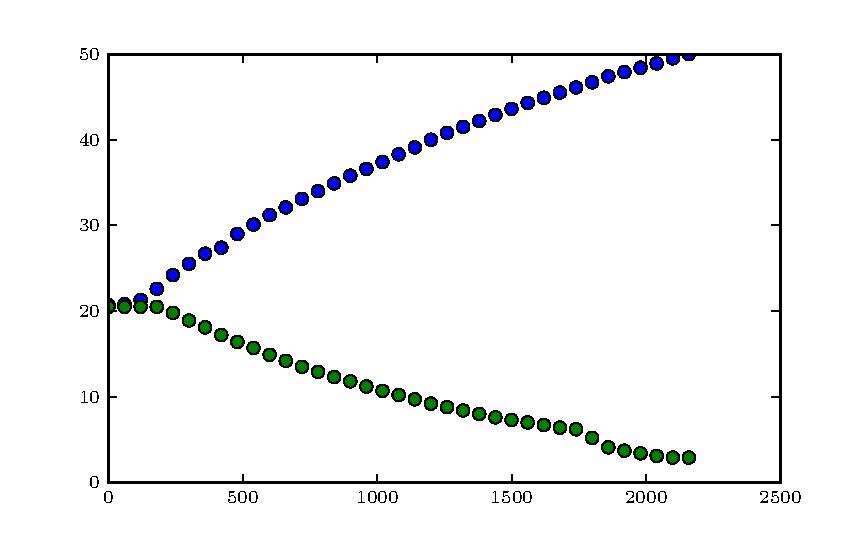
\includegraphics{plot.pdf}
%  \caption{Plot.}
%  \label{fig:plot}
%\end{figure}
\subsubsection{Bestimmung der mittleren freien Weglänge}
Die mittlere freie Weglänge ergibt sich mit Formel \eqref{eqn:freiewegl} zu
\begin{equation*}
	\bar{w} = 1
\end{equation*}

\FloatBarrier
\subsection{Bestimmung der Skalierungen}
Die abgelesenen Werte für die Skalierung der Messung bei $\SI{150}{\celsius}$ sind in 
Tabelle \ref{tab:skalierung_a_2} aufgetragen.
\begin{table}
	\centering
	\caption{Messdaten zur Bestimmung der Grenzspannung $U_\mathrm{G}$.}
	\label{tab:ug}
	\begin{tabular}{cc}
		\toprule
		$U_{\mathrm{B}}$ / $\si{\volt}$ & Abstand / $\si{\centi\meter}$ \\
		\midrule
		0 & 0 \\
		1 & 2.1 \\
		2 & 4.1 \\
		3 & 5.9 \\
		4 & 7.9 \\
		5 & 9.9 \\
		6 & 12.0 \\
		7 & 14.0 \\
		8 & 16.1 \\
		9 & 18.1 \\
		10 & 20.2 \\
		\bottomrule
	\end{tabular}
\end{table}









%%%%%%%%%%%%%%%%%%%%%%%%%%%%%%%%%%%%%%%%%%%%%%%%%%%%%%%%%%%%%%%%%%%%%%%%%%%%%%%%%%%%%%%%%%%%
\FloatBarrier
\subsection{Bestimmung der Ionisationsspannung von Quecksilber}
In Abbildung \ref{fig:ionisation} ist der Auffängerstrom $I_{\mathrm{A}}$ in Abhängigkeit 
von der Beschleunigungsspannung $U_{\mathrm{B}}$ bei einer Gegenspannung von $-\SI{30}{\volt}$ 
aufgetragen. 

